%\documentclass[12pt,a4paper,twocolumn]{report}
\documentclass[12pt]{IEEEtran}
%\usepackage[top=1in, bottom=1in, left=1in, right=1in]{geometry}
\usepackage[utf8]{inputenc}
\usepackage{amsmath}
\usepackage{amsfonts}
\usepackage{amssymb}
\usepackage{graphicx}
\usepackage{mdframed}
\usepackage{multicol}

\title{ECE 520 Final Project}
\author{Christopher Johnson, Joshua Stevens}
\date{April 09, 2014}

\begin{document}

\twocolumn[{\centering
\textbf{\Large Histogram Equalizer\\}
\large \textbf{ECE 520 Final Project\\}
	Christopher Johnson, Joshua Stevens
	\normalsize
	\\[3em]

\begin{mdframed}
\textbf{Project Responsibilities:}\\
csjohns3. Christopher Johnson:\\
${}$\hspace{5em}Input Pipeline, Testbench, Top, Report \vspace*{.5em}\\
jasteve4. Joshua Stevens:\\
${}$\hspace{5em}Output Pipeline/CDF, Testbench, Top, Report\\
\end{mdframed}

%%%%%%%%%%%%%%%%%%%%%%%%%%   3 columns
\begin{multicols}{3}
	\begin{mdframed}
		Delay (ns to run ex)\\ \\
		Clock period: \\ \\
		Cycles: \\
	\end{mdframed}
	
	\begin{mdframed}
		(delay.area)(ns-1.um-2):\\\\\\
	\end{mdframed}

	\begin{mdframed}
		Area: $um^{2}$\\ \\
		Logic:\\ \\
		Memory: N/A\\
	\end{mdframed}
\end{multicols}
%%%%%%%%%%%%%%%%%%%%%%%%%%   END 3 columns

%%%%%%%%%%%%%%%%%%%%%%%%%%   2 columns
\begin{multicols}{2}
	\begin{mdframed}
		Delay (ns to run example)\\
		Clock period: \\
		cycles: \\
	\end{mdframed}
	
	\begin{mdframed}
		1/(delay.area)($ns^{-1}.um^{-2}$)\\
		\\
		\\
	\end{mdframed}
\end{multicols}}]
%%%%%%%%%%%%%%%%%%%%%%%%%%  END 2 columns

\begin{flushleft}
\textbf{\emph{Abstract} - This paper describes a hardware design responsible for improving the contrast of individual frames of a video capture device. The algorithm is based on a histogram equalizer and the hardware is heavily pipelined in order to allow a low clock speed and the ability to quickly process individual images. Using Synopsys Design Vision and Mentor Graphic ModelSim, we prove that it with this module, it is possible to process video at \textbf{REPLACE} $frames/second$ with an area of \textbf{REPLACE} $um^{2}$.}
\end{flushleft}

\section{Introduction}

\begin{flushleft}
When uses a video capturing device, it can be quite common to achieve footage with poor contrast. This is something that can be solved relatively easy using a software histogram equalizer however, this will limit the video capture speed the speed of the software. To alleviate this bottleneck, we have hardware histogram equalizer. Our design is heavily pipelined allowing the clock speed to be quite low while allowing multiple images to be processed at a time. The result is a hardware module that can process video at \textbf{REPLACE} $frames/second$ and an area of \textbf{REPLACE} $m^{2}$. This is significant since this is much smaller and faster than comparative software performing the same function.
\end{flushleft}

\section{Micro-Architecture}

\begin{figure}[htb!]
	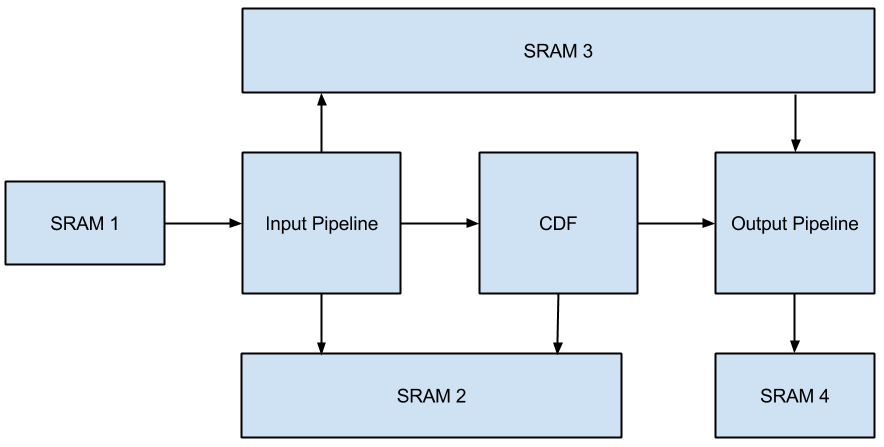
\includegraphics[width=90mm]{System_Overview.png}
	\caption{System Overview}
\end{figure}

\begin{flushleft}
Our overall system is divided into two major stages ("Input Pipeline/CDF Pipeline" and "Output Pipeline") that are individually pipelined and interface through a controller module. These two stages are pipelined such that the "Input Pipeline/CDF Pipeline" module runs in approximately the same time as "Output Pipeline" allowing both modules to run images simultaneously with a minimum number of unused clock cycles.
\end{flushleft}

\subsection*{Input Pipeline}
\begin{flushleft}
This module is responsible for reading pixel values from memory and storing how many times each pixel value occurs to SRAM 2. In order to improve efficiency of this process, a five stage pipeline is used. This allows memory operations to happen in separate cycles from the accumulation stages. This is crucial since it takes 2ns to read or write to the SRAM. In order to keep this pipeline running as quick as possible, three data bypasses were introduced for coping with the 2ns memory write. Finally, this module is responsible for copying the original picture from SRAM 1 to SRAM 3 so "Output Pipeline" will have the image for reference.
\end{flushleft}

\subsection*{CDF Pipeline}
\begin{flushleft}
The sole purpose of this module is to calculate the across all pixel values accumulated in the "Input Pipeline" and load the result to SRAM 2. This pipeline takes the least amount of time to complete however, it cannot run until "Input Pipeline" is complete and "Output Pipeline" cannot run until the CDF is fully calculated. For this reason, we decided to combine the "CDF Pipeline" module with the "Input Pipeline" in our overall system.
\end{flushleft}

\subsection*{Output Pipeline}
\begin{flushleft}

\end{flushleft}

\subsection*{Controller}
\begin{flushleft}
"Controller" handles the signal necessary to start and stop each pipeline. This modules alone provides the capability of running two images through our pipeline simultaneously. To make this possible "Controller" toggles the upper most address bit of each read and write to the SRAM 2. Doing this, our system is able to store one image in the lower half of memory so that "Output Pipeline" can reference the values while "Input Pipeline" simultaneously stores data in the lower half of SRAM 2. Intuitively, we alternate which half of memory is read/written from.
\end{flushleft}

\section{Conclusion}
\begin{flushleft}

"Sed ut perspiciatis unde omnis iste natus error sit voluptatem accusantium doloremque laudantium, totam rem aperiam, eaque ipsa quae ab illo inventore veritatis et quasi architecto beatae vitae dicta sunt explicabo. Nemo enim ipsam voluptatem quia voluptas sit aspernatur aut odit aut fugit, sed quia consequuntur magni dolores eos qui ratione voluptatem sequi nesciunt. Neque porro quisquam est, qui dolorem ipsum quia dolor sit amet, consectetur, adipisci velit, sed quia non numquam eius modi tempora incidunt ut labore et dolore magnam aliquam quaerat voluptatem. Ut enim ad minima veniam, quis nostrum exercitationem ullam corporis suscipit laboriosam, nisi ut aliquid ex ea commodi consequatur? Quis autem vel eum iure reprehenderit qui in ea voluptate velit esse quam nihil molestiae consequatur, vel illum qui dolorem eum fugiat quo voluptas nulla pariatur?"
\end{flushleft}
\end{document}

